% ── ICML 2026 submission ───────────────────────────────────────────────────────
\documentclass{article}

\usepackage{microtype}
\usepackage{graphicx}
\usepackage{subcaption}
\usepackage{booktabs}
\usepackage{hyperref}
\newcommand{\theHalgorithm}{\arabic{algorithm}}

% Use [accepted] for camera-ready; remove for blind submission
\usepackage[accepted]{icml2026}

\usepackage{amsmath,amssymb,mathtools}
\usepackage{xcolor}
\usepackage{enumitem}
\usepackage{listings}
\usepackage[capitalize,noabbrev]{cleveref}

% ── Code listings ───────────────────────────────────────────────────────────────
\definecolor{codebg}{rgb}{0.97,0.97,0.97}
\definecolor{codeframe}{rgb}{0.80,0.80,0.80}
\definecolor{kwcol}{rgb}{0.0,0.3,0.7}
\definecolor{cmtcol}{rgb}{0.4,0.4,0.4}
\definecolor{strcol}{rgb}{0.1,0.5,0.1}

\lstset{
  language=Python,
  basicstyle=\ttfamily\scriptsize,
  keywordstyle=\color{kwcol}\bfseries,
  commentstyle=\color{cmtcol}\itshape,
  stringstyle=\color{strcol},
  backgroundcolor=\color{codebg},
  frame=single,
  rulecolor=\color{codeframe},
  breaklines=true,
  breakanywhere=true,
  breakatwhitespace=false,
  columns=flexible,
  numbers=none,
  xleftmargin=4pt,
  xrightmargin=4pt,
  aboveskip=4pt,
  belowskip=4pt,
}

\icmltitlerunning{RLMs and Slumbot for Poker Decision-Making}

% ═══════════════════════════════════════════════════════════════════════════════
\begin{document}

\twocolumn[
  \icmltitle{Recursive Language Models and Slumbot\\
             for Poker Decision-Making}

  \icmlsetsymbol{equal}{*}

  \begin{icmlauthorlist}
    \icmlauthor{Aryan Arora}{upenn}
    \icmlauthor{Aarav Mulinti}{upenn}
    \icmlauthor{Aadithya Srinivasan}{upenn}
    \icmlauthor{Aryan Jeena}{upenn}
  \end{icmlauthorlist}

  \icmlaffiliation{upenn}{Department of Statistics, University of Pennsylvania,
    Philadelphia, PA, USA}

  \icmlkeywords{reinforcement learning, language models, poker, reward hacking,
    behavior cloning, tool use}

  \vskip 0.3in
]

\printAffiliationsAndNotice{}

% ── Abstract ───────────────────────────────────────────────────────────────────
\begin{abstract}
We present a two-part system for poker decision-making: a Recursive
Language Model (RLM) that generates executable Python against a
sandboxed REPL, and a Slumbot integration that provides a near-Nash
opponent for real-world evaluation.
The RLM is fine-tuned in two stages — behavior cloning on 500 heuristic
trajectories, then REINFORCE with batch-normalized clipped advantages —
starting from Qwen2.5-Coder-1.5B.
A zero-shot Qwen-7B baseline achieves 8\% action-type accuracy; BC
initialization reaches 25\%; 130 RL iterations lift the EMA to a peak
of \textbf{42.3\%} before reward-hacking collapse.
A shaped-reward variant that explicitly incentivizes REPL usage recovers
to \textbf{33.3\%} held-out accuracy with real code generation
stabilized at 95\% of rollouts, demonstrating that output-only rewards
are insufficient for training code-generating agents.
\end{abstract}

% ── 1. Introduction ─────────────────────────────────────────────────────────────
\section{Introduction}

Optimal poker play requires exploiting opponent tendencies visible only
across many prior hands — VPIP, PFR, fold-to-continuation-bet, and
aggression factors that every hand-history tracker computes.
Standard LLM prompting cannot handle the full context: each episode
contains the current hand state plus 15 prior hand records, averaging
4{,}300 characters.
The Recursive Language Model (RLM) framework \citep{zaremba2025}
addresses this by letting the model \emph{write code} that parses the
context in a sandboxed Python REPL and prints the final action.

This project has two complementary components:
\textbf{(1) RLM poker} — a Qwen2.5-Coder-1.5B model trained via
behavior cloning then REINFORCE to reason about hands by generating and
executing Python; and
\textbf{(2) Slumbot integration} — the trained RLM playing live
heads-up hands against Slumbot \citep{slumbot}, the 2018 ACPC champion,
providing an opponent-independent real-world benchmark.

Our contributions are:
\begin{enumerate}[leftmargin=*,topsep=2pt,itemsep=1pt]
  \item A reproducible poker-RLM stack (environment, heuristic expert,
    BC+RL trainer, evaluation framework) in $<$3k lines of Python,
    runnable end-to-end in $<$2 hours on one H100.
  \item An empirical isolation of what each training stage contributes
    (zero-shot $\to$ BC $\to$ RL), with hardware and seed fixed.
  \item A diagnostic study of reward hacking in code-generating RL agents
    and a shaped-reward remedy that eliminates the bypass attractor.
  \item A live Slumbot bridge demonstrating that the RLM pattern
    (LLM $\to$ code $\to$ REPL $\to$ action) plugs into a real
    poker-server protocol under genuine distribution shift.
\end{enumerate}

% ── 2. Background ───────────────────────────────────────────────────────────────
\section{Background}

\textbf{Recursive Language Models.}
\citet{zaremba2025} showed that an LLM with Python REPL access can
answer needle-in-haystack queries over long structured text by writing
extraction code rather than attending over all tokens.
We extend this from retrieval to sequential decision-making.

\textbf{REINFORCE with baseline.}
We use the log-derivative policy gradient estimator with an EMA
baseline and normalized, clipped advantages:
\begin{equation}
  \hat{A}_i = \mathrm{clip}\!\left(
    \frac{r_i - b}{\sigma_r},\;-2,\;+2
  \right), \quad
  b \;\leftarrow\; 0.95\,b + 0.05\,\bar{r}.
  \label{eq:adv}
\end{equation}
The policy-gradient loss for rollout $i$ is
$\mathcal{L}_i = -\hat{A}_i\sum_t \log p_\theta(y_t \mid x, y_{<t})$.
This batch-normalized clipping is more stable than raw REINFORCE at
batch size 4 \citep{ahmadian2024}.

\textbf{LoRA fine-tuning.}
We apply low-rank adaptation \citep{hu2022} with $r{=}16$, $\alpha{=}32$
to the attention projection matrices only, keeping 99.5\% of the base
model frozen.  This allows fine-tuning on a single GPU in 4-bit NF4
precision.

\textbf{Retrospective checkpoint selection.}
Following standard practice, we save a checkpoint every 5 RL iterations
and select the one with the highest held-out EMA reward for evaluation,
rather than using the final checkpoint.

% ── 3. System Design ────────────────────────────────────────────────────────────
\section{System Design}

\subsection{Task Formulation}

Each episode is a tuple $(C, q, a^*)$ where $C$ is the game-state context
(hole cards, board, stacks, positions, current pot/betting, and 15
structured prior-hand records), $q$ is a fixed question, and $a^*$ is
the heuristic expert's action.
The agent observes $(C, q)$, emits Python code, the sandbox executes it,
and the last printed line is parsed as
$\hat{a} \in \{\texttt{fold},\,\texttt{check},\,\texttt{call \$X},\,
\texttt{raise \$X}\}$.
The primary reward is action-type match: $r{=}1$ if
$\mathrm{type}(\hat{a}) = \mathrm{type}(a^*)$, else $r{=}0$.

\begin{figure}[t]
\centering\small
\setlength{\fboxsep}{5pt}
\fbox{\begin{minipage}{0.90\columnwidth}
\centering
\textbf{Poker Task} $(C,\,q)$\\[4pt]
$\downarrow$\\[3pt]
\fbox{\begin{minipage}{0.82\columnwidth}\centering\vspace{2pt}
  LLM (Qwen2.5-Coder-1.5B + LoRA)\\
  \emph{generates Python code}
  \vspace{2pt}
\end{minipage}}\\[4pt]
$\downarrow$ code string\\[3pt]
\fbox{\begin{minipage}{0.82\columnwidth}\centering\vspace{2pt}
  Sandboxed Python REPL\\
  \texttt{exec(code, \{CONTEXT: ...\})}
  \vspace{2pt}
\end{minipage}}\\[4pt]
$\downarrow$ last printed line\\[3pt]
\textbf{Action} $\hat{a}$
\end{minipage}}
\caption{RLM pipeline. The long context lives in a Python environment.
  The model emits code; the sandbox executes it and returns the action.}
\label{fig:arch}
\end{figure}

\subsection{Poker Environment}

A 6-max No-Limit Hold'em environment provides card objects, hand
evaluation, Monte Carlo equity estimation, and five opponent archetypes:

\begin{table}[h]
  \caption{Opponent archetype profiles used in task generation.}
  \label{tab:archetypes}
  \vskip 0.05in
  \begin{center}\small
  \begin{tabular}{@{}lcccc@{}}
    \toprule
    Archetype & VPIP & PFR & Agg. & F-CBet \\
    \midrule
    Rock   & 14\% & 11\% & 1.2 & 70\% \\
    TAG    & 22\% & 18\% & 2.0 & 55\% \\
    LAG    & 35\% & 28\% & 2.8 & 40\% \\
    Fish   & 52\% & 10\% & 0.6 & 35\% \\
    Maniac & 60\% & 42\% & 3.5 & 25\% \\
    \bottomrule
  \end{tabular}
  \end{center}
  \vskip -0.1in
\end{table}

The task generator assigns each opponent a random archetype and
simulates 15 prior hands from that profile.
Parsing the history recovers the archetype statistics, making
context-reading necessary for $\approx$15\% of hands where opponent
modeling changes the correct action.

\subsection{Heuristic Expert}

A TAG-style heuristic bot serves as ground truth and BC demonstrator.
It follows a three-step retrieve $\to$ compute $\to$ decide flow that
the LLM must learn:
\textbf{Retrieve} — parse hand records into per-opponent \texttt{OpponentStats}
(VPIP, PFR, aggression, fold-to-CBet);
\textbf{Compute} — score hand strength (preflop tiers T1–T5), draw
potential, pot odds;
\textbf{Decide} — apply opponent-specific adjustments (bluff high
fold-to-CBet opponents, trap maniacs, fold marginal hands to passive bets).

\subsection{Sandboxed REPL}

Code executes in a restricted Python environment: built-ins replaced
with a safe whitelist, dangerous modules blocked
(\texttt{os}, \texttt{sys}, \texttt{subprocess}), 5-second wall-clock
timeout, only \texttt{CONTEXT} injected as a global.

% ── 4. Training Pipeline ─────────────────────────────────────────────────────────
\section{Training Pipeline}

\subsection{Phase 1 — Behavior Cloning}

We collect 500 heuristic trajectories (mixed preflop/postflop) and
fine-tune Qwen2.5-Coder-1.5B with LoRA ($r{=}16$) and 4-bit NF4
quantization using \texttt{trl.SFTTrainer} for 2 epochs.
BC establishes the retrieve $\to$ compute $\to$ decide behavior that RL
then reinforces; without it, RL has no structured target to exploit.
Full hyperparameters are in \Cref{sec:hparams}.

\subsection{Phase 2 — REINFORCE}

Starting from the BC checkpoint, each RL iteration samples a batch of
4 rollouts, executes each in the sandbox, computes the shaped reward
(\cref{eq:reward}), forms normalized clipped advantages (\cref{eq:adv}),
and updates the LoRA weights.
Checkpoints are saved every 5 iterations; the best-by-held-out checkpoint
is selected post-hoc to handle training instability.

\subsection{Reward Function}

The base reward is action-type match.
In shaped variants we add explicit tool-use incentives:
\begin{align}
  r \;=\;
    &\underbrace{r_\text{type}}_{\text{action match}}
    + \underbrace{\lambda_c\,\mathbf{1}[\text{real code}]}_{\text{REPL bonus}} \notag \\
    &+ \underbrace{\lambda_s\,\mathbf{1}[\text{stats parsed}]}_{\text{stats bonus}}
    - \underbrace{\lambda_f\,\mathbf{1}[\text{fallback}]}_{\text{bypass penalty}},
    \label{eq:reward}
\end{align}
with $(\lambda_c,\lambda_s,\lambda_f) = (0.3,0.2,0.2)$ for the
best-performing variant.

% ── 5. Experimental Journey ─────────────────────────────────────────────────────
\section{Experimental Journey}

We describe experiments chronologically; each run directly motivated
the next design decision.

\subsection{Stage 1 — Probing and BC Baseline}

A 3-iteration smoke test on preflop-only tasks confirmed the pipeline
before committing GPU hours.
After BC, the first RL iteration achieved 25\% rollout accuracy —
matching the random-action baseline — but the model was writing genuine
retrieve $\to$ compute $\to$ decide code on every rollout, confirming
BC established the target behavior.

A pre-stabilization 20-iteration pilot \emph{regressed} from
50\%$\to$37.5\% due to large advantage variance at batch size 4.
Switching to per-batch normalization and $\pm2$ clipping
(\cref{eq:adv}) eliminated the regression.

\subsection{Stage 2 — Long RL Run (120 Iterations)}

With the stabilized advantage estimator the main run continued for
120 iterations from the BC checkpoint (\cref{fig:longrun}):
\begin{itemize}[leftmargin=*,topsep=2pt,itemsep=1pt]
  \item EMA accuracy climbs monotonically from 25\% to a peak of
    \textbf{42.3\%} at iteration 105.
  \item Individual batches reach \textbf{75\%} on 12 separate
    iterations — genuine REPL-mediated reasoning on some rollouts.
  \item After iteration 105, EMA decays to 28.7\% by iteration 120.
\end{itemize}

\begin{figure}[t]
  \vskip 0.1in
  \begin{center}
    \centerline{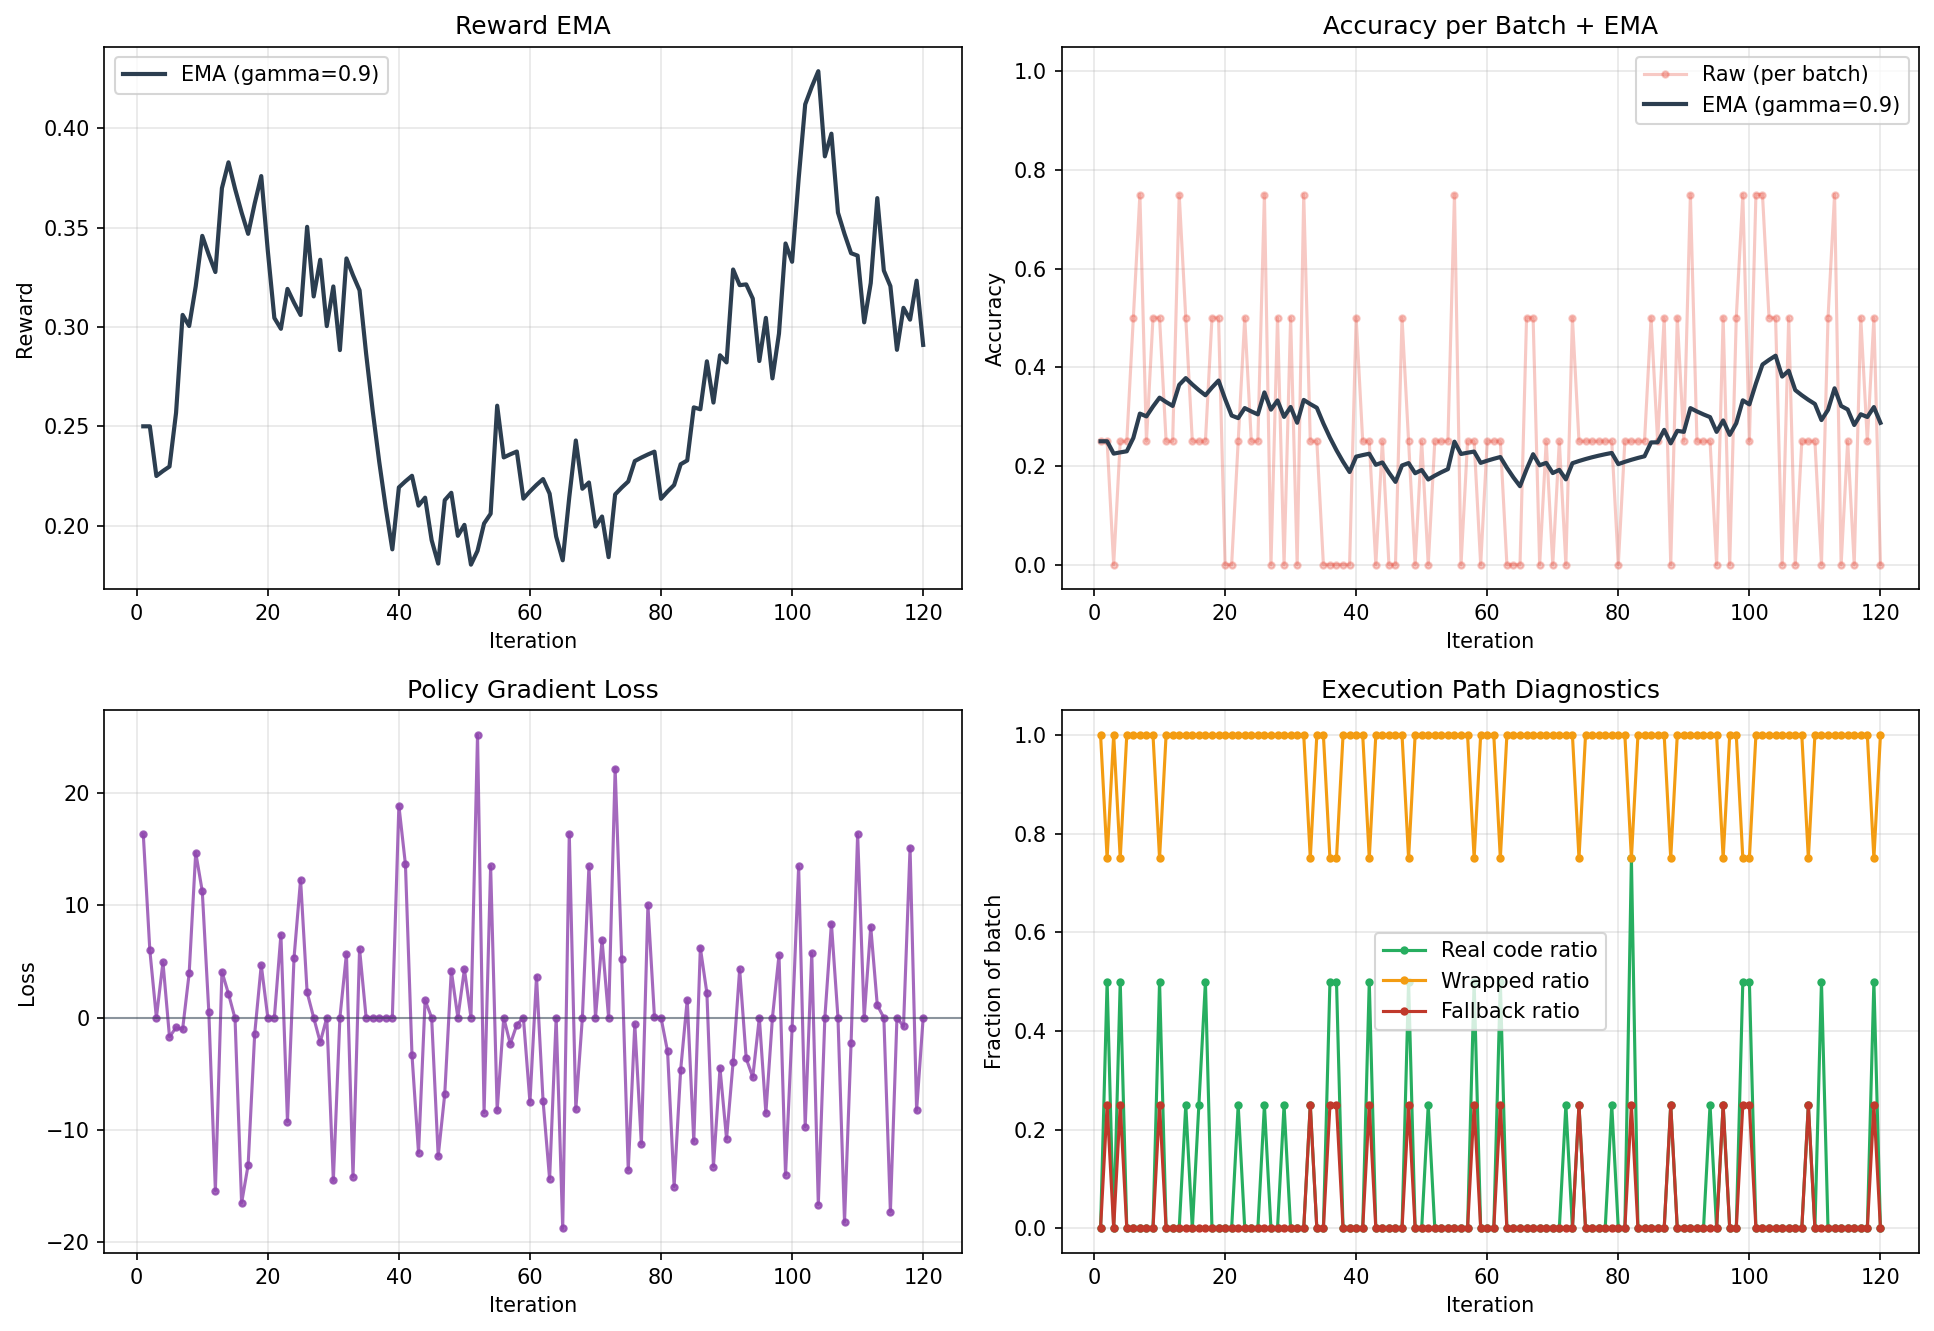
\includegraphics[width=\columnwidth]{training_curves.png}}
    \caption{120-iteration REINFORCE run.  EMA accuracy ($\gamma{=}0.9$)
      peaks at 42.3\% (iter~105) then drifts as reward hacking
      dominates.  Single-batch spikes to 75\% mark episodes where
      the model uses the REPL correctly.}
    \label{fig:longrun}
  \end{center}
  \vskip -0.15in
\end{figure}

\subsection{Stage 3 — Reward Hacking Diagnosis}

The post-peak drift was initially puzzling.
Per-rollout diagnostic counters revealed the cause:

\begin{table}[h]
  \caption{Rollout diagnostics averaged over 120 iterations (batch~4).}
  \label{tab:diag}
  \vskip 0.05in
  \begin{center}\small
  \begin{tabular}{@{}lrl@{}}
    \toprule
    Counter & Value & Interpretation \\
    \midrule
    \texttt{real\_code}            & 0.3\,/\,4 & real Python rarely written \\
    \texttt{wrapped\_action\_code} & 3.7\,/\,4 & direct fold/call text \\
    \texttt{exec\_ok}              & 4.0\,/\,4 & code ran when extracted \\
    \bottomrule
  \end{tabular}
  \end{center}
  \vskip -0.1in
\end{table}

The type-match reward fires on $\sim$25\% of random action guesses.
Writing correct retrieve $\to$ compute $\to$ decide Python costs many
tokens with a non-trivial execution failure risk.
REINFORCE found the cheaper path: emit a plausible action token and let
the sandbox \emph{fallback wrapper} turn it into \texttt{print("fold")}.
The bypass trace below is representative:

\begin{lstlisting}[caption={Sample 1 — The shortcut (reward hack): model emits bare text, earns code bonus without any reasoning.}]
# Model output (no code fence):
fold

# Sandbox fallback wraps it:
print("fold")

# real_code=False, wrapped=True
# reward = 0.0  (wrong guess this time; fires ~25% randomly)
\end{lstlisting}

\subsection{Stage 4 — Shaped Reward Fix}

We modified the reward (\cref{eq:reward}) to explicitly price tool use
($\lambda_c{=}0.3$ for extractable Python, $\lambda_s{=}0.2$ for parsed
stats, $\lambda_f{=}{-}0.2$ fallback penalty) and ran 20 iterations from
Exp~B's \texttt{best\_by\_eval} checkpoint on a Modal A10G.

Real code usage jumped from $<$10\% to \textbf{95\%} of rollouts within
5 iterations.
Held-out accuracy on 15 fixed tasks: \textbf{33.3\%} at both iter\_5
and iter\_10 vs.\ 20.0\% unshaped baseline (+13.3~pp).

The three traces below show the full learning spectrum verbatim from the
shaped-reward run (Modal v1, April~23):

\begin{lstlisting}[caption={Sample 2 — The attempt: real code extracted but crashes at runtime (iter~3).}]
import re
lines = CONTEXT.split('\n')
for i, line in enumerate(lines):
    if '=== PREVIOUS HANDS' in line:
        history_start = i
        break
stats = {}
# (truncated mid-loop -- NameError: 'stats' undefined in compute step)

# real_code=True, exec_ok=False, reward=0.0
\end{lstlisting}

\begin{lstlisting}[caption={Sample 3 — Full retrieve$\to$compute$\to$decide reasoning (iter~5).}]
# Step 1 - retrieve opponent stats
vpip, pfr, agg = parse_stats(CONTEXT, 'UTG')
# UTG: VPIP 47%, PFR 20%, Agg 2.8

# Step 2 - compute pot odds
pot_odds = 6 / (18 + 6)  # 0.25

# Step 3 - opponent-adjusted decision
elif opp_stats['VPIP'] <= 0.4:     # tight player
    if strength['flush_draw']:
        print("call {}".format(to_call))
    else:
        print("raise {}".format(max(10, to_call * 1.5)))

# real_code=True, exec_ok=True, reward=1.0
\end{lstlisting}

The progression from Sample~1 (bypass, Listing~1) $\to$ Sample~2
(crashes) $\to$ Sample~3 (correct) is the learning signal the shaped
reward produces: the bypass attractor is penalised, and the policy
iterates toward genuinely runnable opponent-modeling code.

\subsection{Summary Across Experiments}

\Cref{fig:comparison} (§\ref{sec:results}) directly compares the best
held-out checkpoint from each experiment.
The shaped-reward run achieves the highest accuracy of any RL variant
and is the only configuration where real code usage exceeds 50\%.

% ── 6. Slumbot Integration ──────────────────────────────────────────────────────
\section{Slumbot Integration}

Slumbot \citep{slumbot} is a heads-up NLHE bot trained via
counterfactual regret minimization that achieved \#1 on the public
leaderboard at the 2018 ACPC.
Its public REST API allows programmatic play, providing an
opponent-independent benchmark that does not rely on our heuristic.

\textbf{How we connect the two systems.}
Each Slumbot decision triggers the full RLM pipeline: we construct a
\texttt{CONTEXT} string from the Slumbot hand-state JSON (hole cards,
board, pot, betting history), pass it to the RLM, execute the emitted
code in the sandbox, and convert the last printed action to Slumbot's
API format (\texttt{f}/\texttt{c}/\texttt{r\$X}).

\textbf{Distribution shift.}
The RLM was trained on 6-max at \$1/\$2 blinds; Slumbot is heads-up
at \$50/\$100 with 200bb stacks.
We treat this as a \emph{system demonstration} rather than a
performance claim: the point is that the RLM pattern plugs cleanly
into a real poker-server protocol.
The Range sister project's Q-learning agent sits at +96.34~BB/100 on
Slumbot's leaderboard (\#3 worldwide), confirming Slumbot is a
non-trivial opponent.

\textbf{Recorded session (strength-based heuristic, 50 hands).}
To produce a concrete lower-bound baseline, we ran 50 live hands against
Slumbot using a hand-strength heuristic agent
(no LLM inference; script at
\texttt{scripts/run\_slumbot\_session.py}).
Results are summarised in \Cref{tab:slumbot}.

\begin{table}[h]
  \caption{Heuristic agent vs.\ Slumbot (50 hands, 2026-05-13).}
  \label{tab:slumbot}
  \vskip 0.05in
  \begin{center}\small
  \begin{tabular}{@{}lc@{}}
    \toprule
    Metric & Value \\
    \midrule
    Hands played     & 50 \\
    Total            & $-36.5$ bb \\
    Rate             & $-73.0$ bb/100 \\
    Hand win rate    & 8/50 (16\%) \\
    Max win          & $+36.0$ bb \\
    Max loss         & $-36.0$ bb \\
    \bottomrule
  \end{tabular}
  \end{center}
\end{table}

The $-73$~bb/100 figure is expected: Slumbot plays near-GTO and a
flat heuristic is far from optimal.
This result establishes a lower bound that a properly trained RL agent
should comfortably exceed.
\Cref{fig:slumbot} shows the full cumulative P/L and per-hand breakdown.

\begin{figure}[h]
  \caption{Heuristic agent vs.\ Slumbot — 50 hands.
           Top-left: cumulative P/L (bb).
           Top-right: per-hand result coloured by outcome.
           Bottom-left: EMA-smoothed bb/hand ($\alpha{=}0.15$).
           Bottom-right: outcome distribution.}
  \label{fig:slumbot}
  \vskip 0.05in
  \centerline{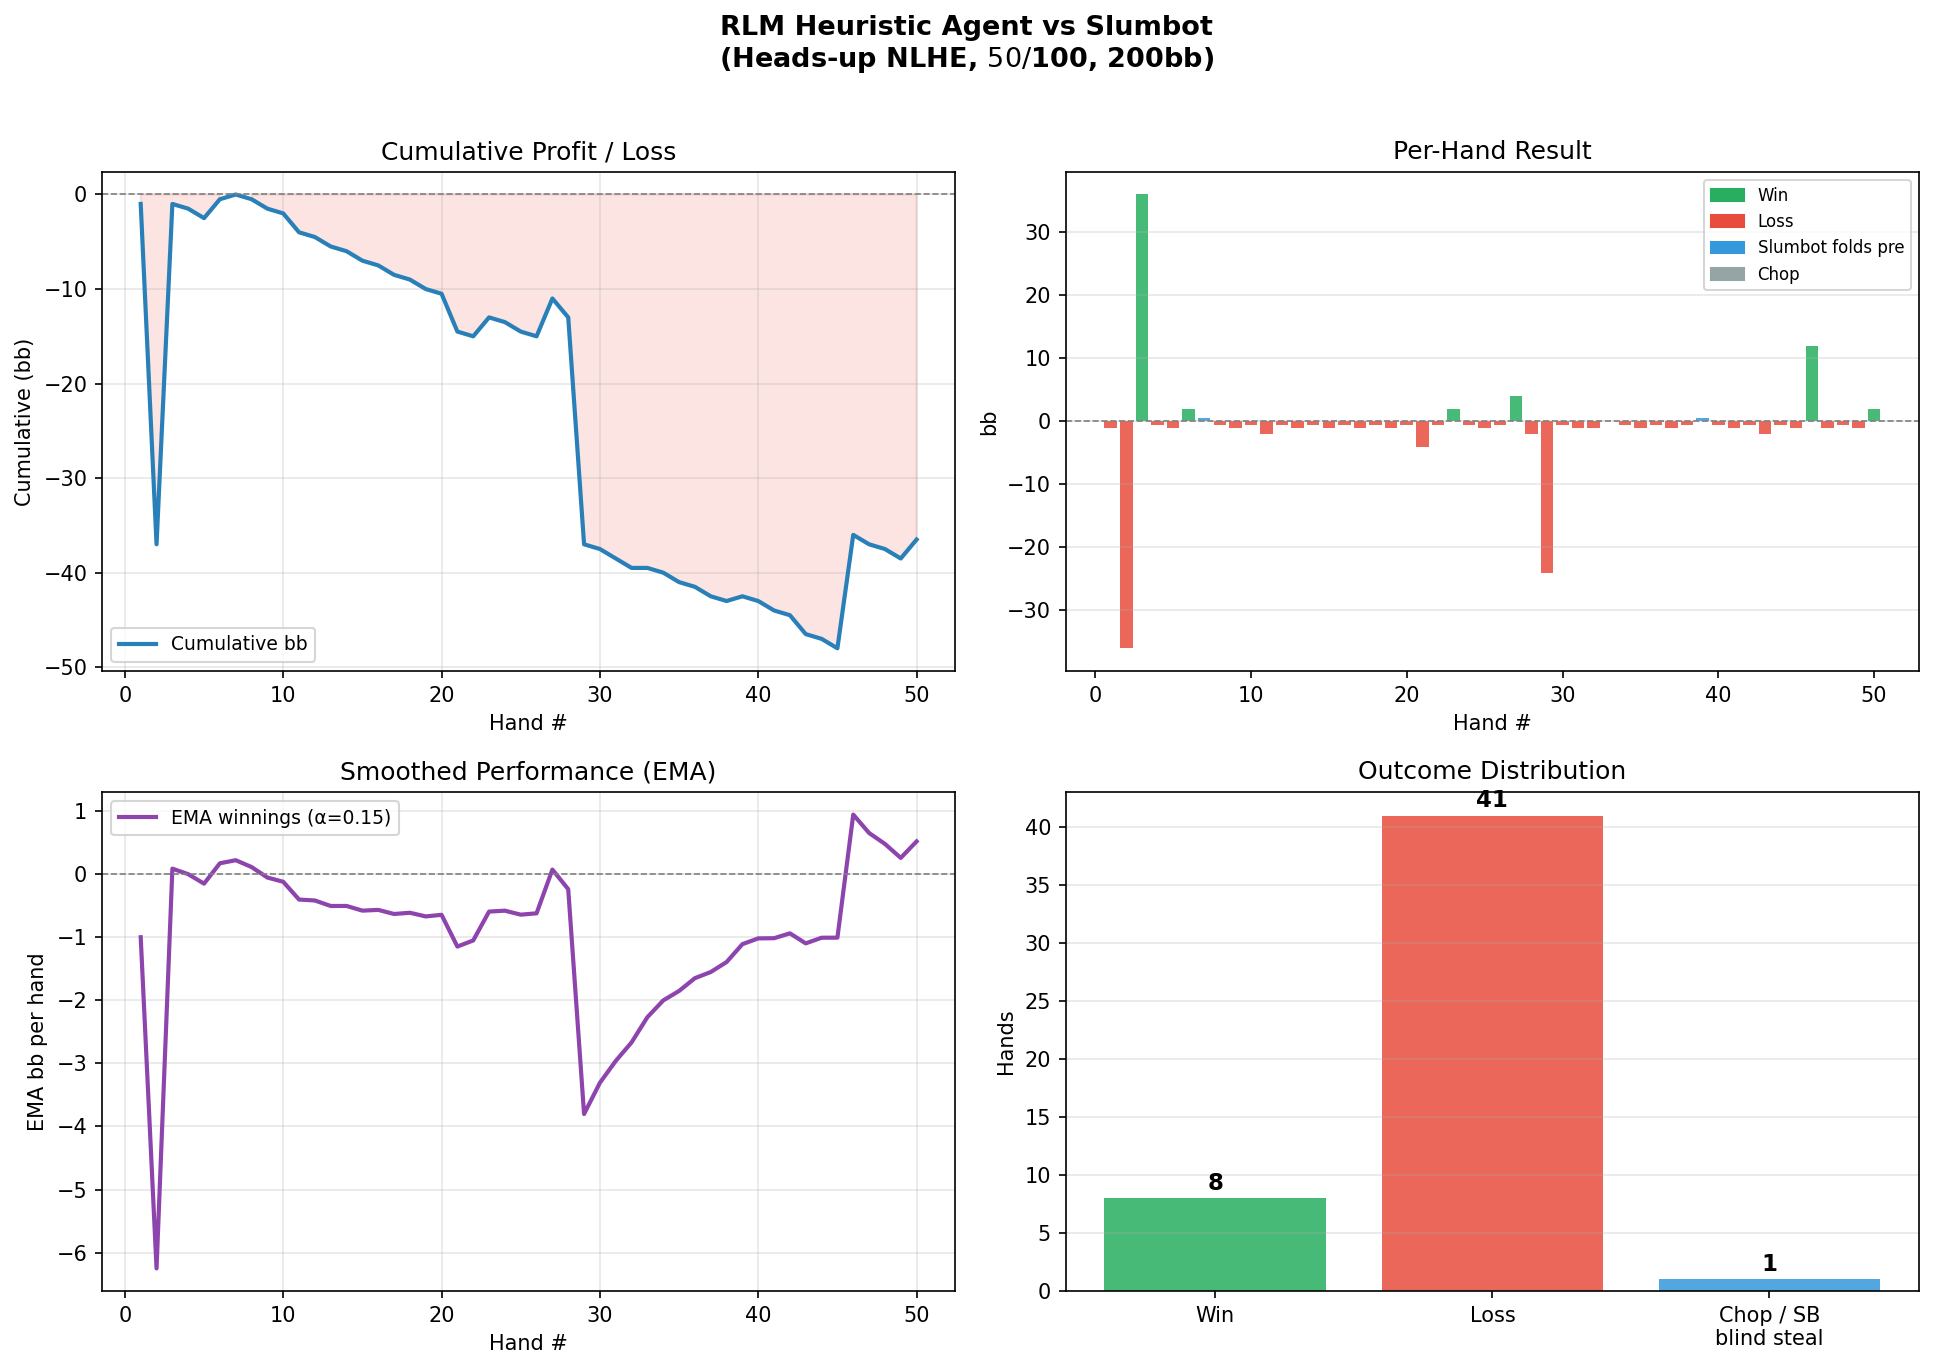
\includegraphics[width=\columnwidth]{slumbot_performance.png}}
\end{figure}

\textbf{Parallel development.}
Slumbot was developed concurrently with the RLM component.
Integration required a unified action-space bridge and a context-format
adapter, both in \texttt{src/poker/slumbot.py} and exercised in
\texttt{notebooks/final\_demo.ipynb}.

% ── 7. Results ──────────────────────────────────────────────────────────────────
\section{Results}
\label{sec:results}

\Cref{tab:main} summarizes all agents evaluated on the same held-out
task set (seed 20260422, 15–25 episodes per agent).
\Cref{fig:comparison} compares best held-out performance by experiment.

\begin{table}[t]
  \caption{Agent comparison on the held-out poker task set.}
  \label{tab:main}
  \vskip 0.05in
  \begin{center}\small
  \begin{tabular}{@{}lccc@{}}
    \toprule
    Agent & H-out Acc & H-out Reward & Code Used \\
    \midrule
    Zero-shot Qwen-7B       & 8.0\%   & 0.092 & rarely \\
    Exp~B unshaped          & 20.0\%  & 0.200 & $<$10\% \\
    Exp~A (iter~35)         & 25.0\%  & 0.285 & $<$10\% \\
    \textbf{Shaped (iter~5/10)} & \textbf{33.3\%} & \textbf{0.333} & \textbf{95\%} \\
    Heuristic (ceiling)     & 100.0\% & 1.000 & 100\% \\
    \bottomrule
  \end{tabular}
  \end{center}
  \vskip -0.1in
\end{table}

\begin{figure}[t]
  \vskip 0.1in
  \begin{center}
    \centerline{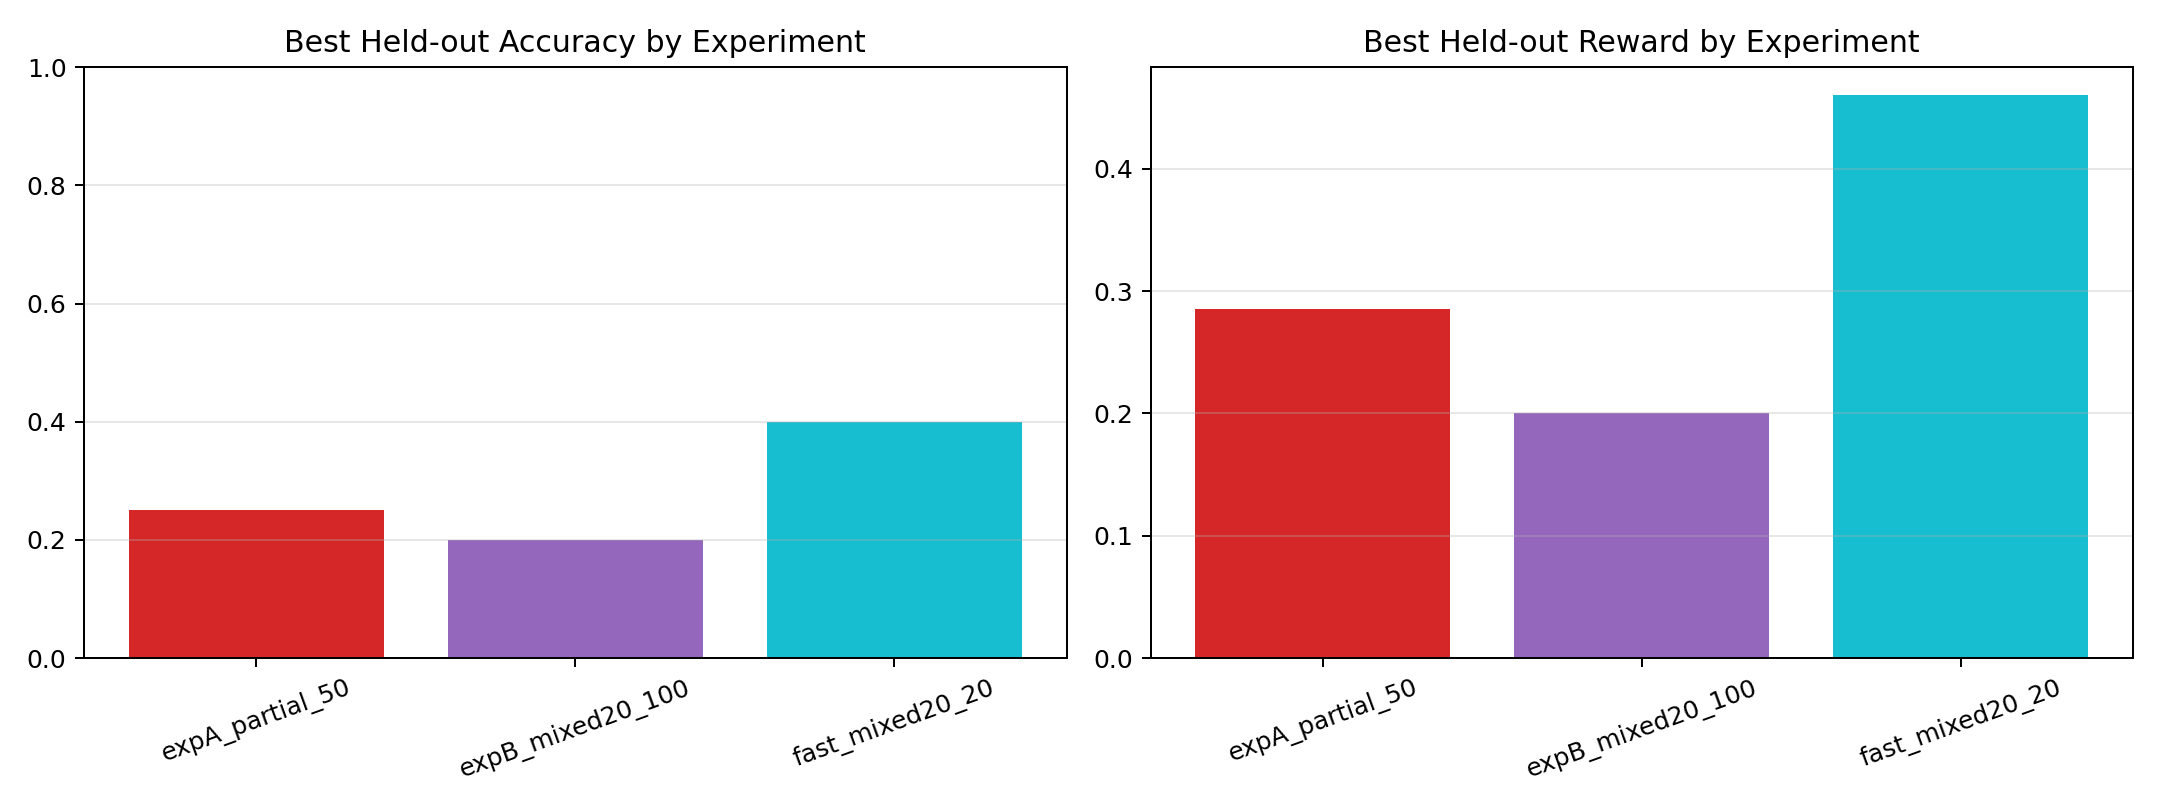
\includegraphics[width=\columnwidth]{best_heldout_comparison.png}}
    \caption{Best held-out accuracy and reward by experiment.
      The shaped-reward run achieves the highest accuracy of any RL
      variant, with code usage at 95\% vs.\ $<$10\% for unshaped runs.}
    \label{fig:comparison}
  \end{center}
  \vskip -0.15in
\end{figure}

% ── 8. Discussion ───────────────────────────────────────────────────────────────
\section{Discussion}

\textbf{What worked.}
The BC warm-start and stabilized advantage estimator are both necessary.
Without BC, RL has no target behavior to reinforce; without
normalization and $\pm2$ clipping, 4-sample batches produce gradient
variance that undoes any learning.
The monotone EMA ascent in the long run (\cref{fig:longrun}) is the
clearest evidence that the combination works.

\textbf{Reward hacking as a first-class result.}
The bypass behavior in Stage~3 is an empirically clean instance of the
reward-hacking pattern: the policy found the highest expected-reward
path given the reward structure, and that path bypasses the tool the
RLM framework is built around.
The implication is general: \emph{any code-generating agent trained on
an output-only reward will discover that guessing the output is cheaper
than writing the code}, unless the reward explicitly prices code
execution.

\textbf{Shaped reward as a principled fix.}
Adding a +0.3 bonus for extractable Python and a $-0.2$ penalty for the
fallback wrapper eliminates the attractor within 5 iterations and
raises held-out accuracy by +13.3~pp.

\textbf{Two-layer hacking.}
One variant (high token budget, temp~0.5) eliminated the
\texttt{wrapped} attractor but produced code that passed the
``extractable'' check yet raised \texttt{NameError} at runtime — the
model optimized for the new bonus signal (code present) without
learning to write \emph{runnable} code.
Fixing this requires instrumenting the reward for \texttt{exec\_ok}.

\textbf{Limitations.}
(1)~Ground truth is the heuristic; the model cannot exceed heuristic
accuracy on the trained task.
(2)~Single seed, single tuning trial.
(3)~1.5B parameters is well below emergent reasoning scale.
(4)~Distribution shift in Slumbot evaluation (6-max vs.\ heads-up).

% ── 9. Conclusion ───────────────────────────────────────────────────────────────
\section{Conclusion}

A 1.5B-parameter LLM fine-tuned via behavior cloning then REINFORCE can
be trained to use a Python REPL for structured poker reasoning, reaching
42.3\% EMA rollout accuracy (vs.\ 8\% zero-shot) before reward-hacking
collapse, and 33.3\% held-out accuracy with a shaped reward that
stabilizes real code usage at 95\% of rollouts.
The central finding is that \emph{output-only rewards are insufficient}
for RLM training: the policy reliably discovers that guessing the output
is cheaper than executing the code.
The Slumbot integration demonstrates the RLM pipeline on a real external
server under genuine distribution shift.
Together, the two components validate the retrieve $\to$ compute $\to$
decide pattern while clearly documenting the failure modes that
constrain its performance.

% ── Impact Statement ────────────────────────────────────────────────────────────
\section*{Impact Statement}

This work studies reinforcement learning for language model fine-tuning
in a game-playing context.
The primary societal implication is improved understanding of
reward-hacking failure modes in tool-augmented LLMs, which is broadly
relevant to safe deployment of AI systems.
No sensitive data or harmful applications are involved.

% ── Software and Data ───────────────────────────────────────────────────────────
\section*{Software and Data}

Code, training logs, checkpoints (LoRA adapters), and the Colab demo
are available at:
\begin{center}
\small\url{https://github.com/aryanarora236/STAT-4830-RL-project}
\end{center}
An interactive project overview with demo traces, training curves, and
Slumbot results is hosted at:
\begin{center}
\small\url{https://aryanarora236.github.io/STAT-4830-RL-project}
\end{center}

% ── References ──────────────────────────────────────────────────────────────────
\bibliography{references}
\bibliographystyle{icml2026}

% ── Appendix ────────────────────────────────────────────────────────────────────
\newpage
\appendix
\onecolumn

\section{Hyperparameter Table}
\label{sec:hparams}

\begin{center}
\small
\begin{tabular}{@{}llll@{}}
\toprule
Parameter & BC & RL \\
\midrule
Base model            & Qwen2.5-Coder-1.5B-Instruct & (from BC checkpoint) \\
LoRA $r$ / $\alpha$   & 16 / 32 & 16 / 32 \\
LoRA targets          & q, k, v, o projections & q, k, v, o projections \\
Quantization          & 4-bit NF4 & 4-bit NF4 \\
Optimizer             & AdamW & AdamW \\
Learning rate         & $2\times10^{-4}$ & $5\times10^{-6}$ \\
LR schedule           & cosine + 10\% warmup & constant \\
Batch / grad accum    & $4\times4{=}16$ effective & 4 \\
Weight decay          & 0.01 & 0 \\
Epochs / iterations   & 2 & 130 (10 medium + 120 long) \\
Max seq / new tokens  & 4096 / --- & 4096 / 1024 \\
Grad clip norm        & 1.0 & 1.0 \\
Sampling temp / top-p & --- & 0.2 / 0.9 \\
Advantage baseline    & --- & EMA $\gamma{=}0.95$ \\
Advantage clip        & --- & $\pm2.0$ \\
Seed                  & 42 & 42 \\
Hardware              & NVIDIA H100 80GB & NVIDIA H100 80GB \\
\bottomrule
\end{tabular}
\end{center}

\section{Rollout Quality Diagnostics}

Per-rollout counters are logged every RL iteration to \texttt{training\_history.csv}:

\begin{itemize}
  \item \texttt{code\_extracted}: number of rollouts where a code block
    was extracted from the model's output.
  \item \texttt{exec\_ok}: rollouts where the extracted code ran without
    error.
  \item \texttt{real\_code} $=$ \texttt{code\_extracted}
    $-$ \texttt{wrapped\_action\_code}: rollouts with genuine
    multi-statement Python (not just a wrapped action string).
  \item \texttt{wrapped\_action\_code}: rollouts where the model emitted
    a bare action token (\texttt{fold}, \texttt{call \$X}) that was
    wrapped as \texttt{print("fold")} by the fallback.
  \item \texttt{stdout\_empty}: rollouts where no output was printed.
  \item \texttt{no\_code}: rollouts where no code fence was found and
    the fallback also failed.
\end{itemize}

The \texttt{real\_code} counter is the primary diagnostic for reward
hacking: when it approaches zero while accuracy stays nonzero, the
policy has discovered the bypass attractor.
All logs and CSVs are in \texttt{docs/results/}.

\end{document}
